\documentclass[a4paper,10pt]{article}

% standard packages
\usepackage[utf8]{inputenc}
\usepackage[english]{babel}
\usepackage{csquotes}
\usepackage{geometry}
\usepackage{graphicx}
\usepackage[textsize=footnotesize]{todonotes}

% This is needed for multiple bib-files
% \usepackage[
% 	sortcites=true,
% 	backend=bibtex,
% 	style=ieee,
% 	defernumbers=true,
% ]{biblatex}
% \addbibresource{references.bib} % The name of your bibliography file

% load macros (section title can be changed here)
% section title macros (can be changed)
\newcommand{\insertProjectFundingSchemeTitle}{Project Funding Scheme:}
\newcommand{\insertProjectShortSummaryTitle}{Short Summary:}

% other macros (do not change)
\makeatletter

\newcommand\projectCode[1]{\renewcommand{\insertProjectCode}{#1}}
\newcommand\insertProjectCode{\@latex@error{No \noexpand\projectCode given}\@ehc}

\newcommand\projectTitle[1]{\renewcommand{\insertProjectTitle}{#1}}
\newcommand\insertProjectTitle{\@latex@error{No \noexpand\projectTitle given}\@ehc}

\newcommand\projectPIs[1]{\renewcommand{\insertProjectPIs}{#1}}
\newcommand\insertProjectPIs{\@latex@error{No \noexpand\projectPIs given}\@ehc}

\newcommand\projectFundingScheme[1]{\renewcommand{\insertProjectFundingScheme}{#1}}
\newcommand\insertProjectFundingScheme{\@latex@error{No \noexpand\projectFundingScheme given}\@ehc}

\newcommand\projectShortSummary[1]{\renewcommand{\insertProjectShortSummary}{#1}}
\newcommand\insertProjectShortSummary{\@latex@error{No \noexpand\projectShortSummary given}\@ehc}

%\newcommand\insertProjectHeader{
%  \noindent\hrulefill\\[.5em]
%  \noindent\llap{\fbox{\bfseries\insertProjectCode}\hspace{1em}}{\Large\bfseries\insertProjectTitle} \\[.5em]
%  PIs: \insertProjectPIs\\
%  \null\hrulefill \\[.5em]
%  \begin{tabular}{@{}ll}
%    {\bfseries\insertProjectFundingSchemeTitle} & \insertProjectFundingScheme \\[.5em]
%    {\bfseries\insertProjectShortSummaryTitle} & \insertProjectShortSummary
%  \end{tabular}\\[.5em]
%  \null\hrulefill
%}

\usepackage{tabularx}

\newcommand\insertProjectHeader{
  \noindent\hrulefill\\[.5em]
  \noindent\llap{\fbox{\bfseries\insertProjectCode}\hspace{1em}}{\Large\bfseries\insertProjectTitle} \\[.5em]
  PIs: \insertProjectPIs\\
  \null\hrulefill \\[.5em]
  \begin{tabularx}{\textwidth}{@{} l X @{}}
    {\bfseries\insertProjectFundingSchemeTitle} & \insertProjectFundingScheme \\[.5em]
    {\bfseries\insertProjectShortSummaryTitle} & \insertProjectShortSummary
  \end{tabularx}\\[.5em]
  \null\hrulefill
}

\makeatother



%%%%%%%%%%%%%%%%%%%%%%%%%%%%%%%%%%%%%%%%%%%%%%%%%%%%%%%%%%%%%%%%%%%%%%%%%%%%%%%%
% PLEASE NOTE THE FOLLOWING LENGTH RESTRICTION:
% - no more than 4 pages (incl. publications). 
% - no more than 8 pages (incl. publications) in the exceptional case that you apply for two positions
%%%%%%%%%%%%%%%%%%%%%%%%%%%%%%%%%%%%%%%%%%%%%%%%%%%%%%%%%%%%%%%%%%%%%%%%%%%%%%%%

\newcommand{\bibfilename}{mrabbrev,mybibfile} % <- replace 'mybibfile' with basename of your bibfile

\usepackage[labeled,resetlabels]{multibib}
\newcites{P}{{\normalsize  Publications of PIs and project members}}
\newcites{O}{{\normalsize  Publications of other researchers}}


%%%%%%%%%%%%%%%%%%%%%%%%%%%%%%%%%%%%%%%%%%%%%%%%%%%%%%%%%%%%%%%%%%%%%%%%%%%%%%%%
% FILL OUT PROJECT INFORMATION

%%%%% PROJECT CODE
% Please assign your planned project to one Application Area or Emerging Field of MATH+.
% Code "AA1": Application Area 1 (Life Sciences)
% Code "AA2": Application Area 2 (Materials, Light, Devices)
% Code "AA3": Application Area 3 (Networks)
% Code "AA4": Application Area 4 (Energy and Markets)
% Code "EF1": Emerging Field 1 (Extracting Dynamical Laws from Complex Data)
% Code "EF2": Emerging Field 2 (Digital Shapes)
% Code "EF3": Emerging Field 3 (Model-Based Imaging)
% Code "EF4": Emerging Field 4 (Particles and Agents)
% Code "EF5": Emerging Field 5 (Concepts of Change in Historical Processes)
\projectCode{AA2}

%%%%% PROJECT TITLE
% e.g., Deep learning in Berlin administrations
\projectTitle{Multi Material Electocatalysis II}
%%%%% PIs / Applicants
% Project _heads_ only!
% In case a doctoral researcher is to be selected for a position in the project, 
% applicants must indicate with "*" which PI will act as authorized PhD-supervisor. 
% Form: initial dot lastname, initial dot lastname
\projectPIs{J. Fuhrmann, M. Landstorfer}

%%%%% REQUESTED STAFF
% Please use the following code for the position you request:
% Category A)	Full positions (100% E13) for 2 years, 
% Category B)	75% positions (E13) for 3 years (for projects in AAs and EFs only). 
% If you already know whom you intend to hire, please include the name such as "Category A (Dr. Angela Merkel); Start: 1 JAN 2021"
% In this case, please also include the CV of this person as an additional document in your proposal.
\projectFundingScheme{Category A (Dr. Rüdiger Müller); Start: 1 JAN 2021}

%%%%% SHORT SUMMARY
% Please add a short summary of your project using a maximum of 100 words or 5 lines!!!
\projectShortSummary{Complex, multi-materal electrocatalysts are crucial in many
  applications relevant for the energy transition. Their model based understanding
  will increase the efficiency  and scalability  of electrocatalytic processes.
  Building on the results of the first project period focused on
  thermodynamic equilibrium, modeling and numerical methods  shall be extended to the non-equilibrium case of
  complex surface reactions.
}

%%%%%%%%%%%%%%%%%%%%%%%%%%%%%%%%%%%%%%%%%%%%%%%%%%%%%%%%%%%%%%%%%%%%%%%%%%%%%%%%
% MAIN CONTENT

\begin{document}

\insertProjectHeader


\subsection*{Extended Synopsis of the Proposal}

\paragraph{Background}
% Please include here:
% - Account of the problem
% - Motivation
% - Background
% - State of the art of research in this area
% - Preliminary work by the PIs


% - Account of the problem

The pivotal strategic importance of technologies based on electrocatalytic reactions is underlined in the recently approved National Hydrogen Strategy of the German Federal Government.  This initiative grants hydrogen, and in particular ``green hydrogen'' created with renewable energy a strategic role in the decarbonization of the economy as an energy carrier, an energy storage option, a sector coupling technology, a precursor for the chemical industry and a means for CO2 emission reduction in various industrial processes.
As a part of this strategy, the creation of hydrogen from electrical energy in electrolyzers and the reverse process -- the recovery of electrical energy from hydrogen in fuel cells -- are seen as indispensable technologies whose development shall be supported by R\&D investments and market incentives.
%
Both technologies are based on electro-catalytic reactions. Production and utilization of hydrogen are just two examples for this class of reactions, other electro-catalytic reactions are fundamental in post lithium batteries, material synthesis and other fields.

% - Motivation
The main driving forces for the rapid development of these technologies are (i) the synthetization of new electrode and electrolyte materials (e.g. ionic liquids and perovskites) (ii) the fabrication of nano-structured and composite electro-catalyitc surfaces (multi-material catalysts) and (iii) material and operational optimization. Central goal is to reduce cost, the main issue of large scale electro-catalysis due to high amount of expensive raw materials which are yet required (especially Pt and Pd). The Berlin based cluster of excellence UniSysCat, for example, searches for substitutions of these expensive materials.

% - Background
Investigations of electro-catalytic reactions on new materials  
are carried out by a number of  experimental techniques,  e.g.
RRDE    (Rotating   Ring    Disc   Electrode),   
% DEMS   (Differential Electrochemical  Mass  Spectroscopy), 
CV  (Cyclic  Voltammetry),  
STM (Scanning Tunneling Microscopy), 
% EQCM (Electrochemical Quartz Crystal Microbalance), 
SEM (Scanning  Electrochemical Microscopy),
AFM (Atomic Force Microscopy), 
EIS (Electrochemical Impedance Spectroscopy).

% - State of the art of research in this area

In order to interpret the experimental results, and to understand, predict and optimize electrocatalytic systems, various mathematical models have to be used. Depending on the level of complexity, modeling results can be expressed using analytic expressions or need to be obtained via numerical simulation. Recent research by internationally leading groups more and more focuses on the interplay between mass transport, reactions and the electric field on the nanoscale, resolving double layer effects in order to support expiermental interpretation \cite{lin2019understanding,tan2018double,eden2019modeling,bohra2019modeling}.

All these approaches are based on homogeneous interfaces with no variation in their spatial structure. Especially they do not take into surface inhomogenities, which lead to variations on the electrochemical activity.

% - Preliminary work by the PIs


WIAS research group RG3 represented by PI J. Fuhrmann contributes to the numerical modeling and simulation of electrochemical systems. This includes  the derivation of a thermodynamically consistent finite volume method \cite{JF2016} for the electrolyte models \cite{DGL2014,VagnerEtAl2019}, implementations in Julia\cite{VoronoiFVM} and C++, as well as convergence investigations for different flux thermodynamically consistent flux expressions.   %implementing the model 
 %A similar discretization approach is used for the simulation of solid oxide electrolytes \cite{VagnerEtAl2019}. Convergence investigations for different flux thermodynamically consistent flux expressions of finite volume schemes for unipolar drift-diffusion models have been performed in \cite{CCFG2020}, see also Fig. \ref{fig:fv}, left. The finite volume method for ion transport has been coupled to a pressure robust Navier-Stokes solver for electrolyte flow \cite{FGLMMSpringer2019,FuhrmannEtAlECActa2019}, see also Fig. \ref{fig:fv}, right.
%The Julia language allows to utilize forward mode automatic differentiation to significantly reduce the implementation effort for strongly nonlinear problems reducing to reduce code complexity compared to C++ and to allow for easy distribution of the code based on a modern package management system.  The computational results in \cite{CCFG2020,VagnerEtAl2019} have been obtained by the new Julia package for finite volume methods \cite{VoronoiFVM} developed by the PI.

WIAS research group RG7 represented by PI M. Landstorfer is active in the development of mathematical models for electrochemical systems.  A seminal result is a comprehensive electrolyte model which provides an accurate description of the electrochemical double layer and yields broad accordance to experimental data of single crystal electrodes. Based on this, thermodynamically consistent boundary conditions for electrochemical reactions at electrode surfaces have been developed \cite{DGM2013,DGL2014,Landstorfer2016187,landstorfer2017boundary}.

Recently published work\cite{JES}, supported by Math+ within the project MultECat, provides first results on modeling, simulation and validation of electrochemical interfaces on polycrystalline materials (see Fig. \ref{fig:JES}). In addition a methodological approach to handle realistic multi-material surfaces was developed, allowing for a stochastic description of polycrystalline surfaces. Additional results on Debye--Hückel theory, concentration dependent susceptibilities, and electrolyte transport are in the final stage of publication. % HIER DIE ARBEITEN IN PREP HIn

\begin{figure}
  \centering
  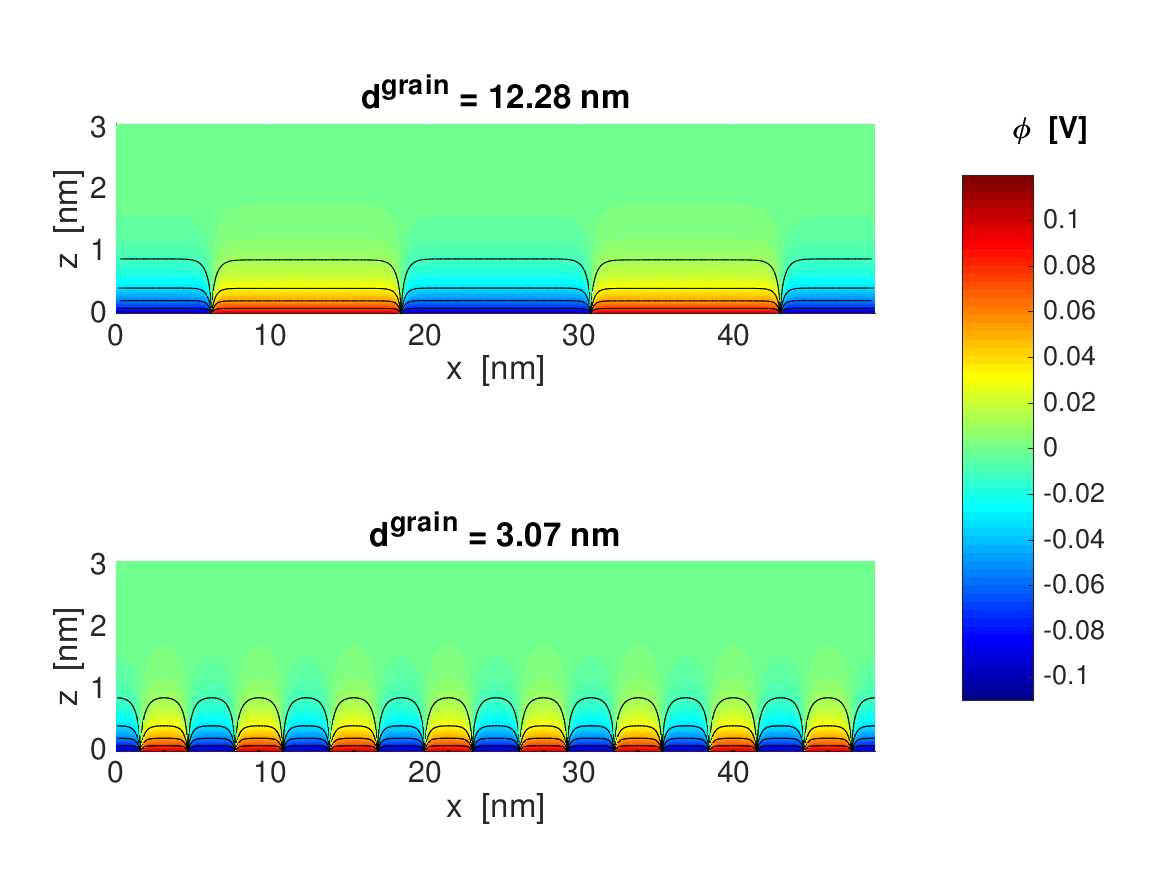
\includegraphics[width=0.45\textwidth]{phi_poly2d_gran.pdf}
  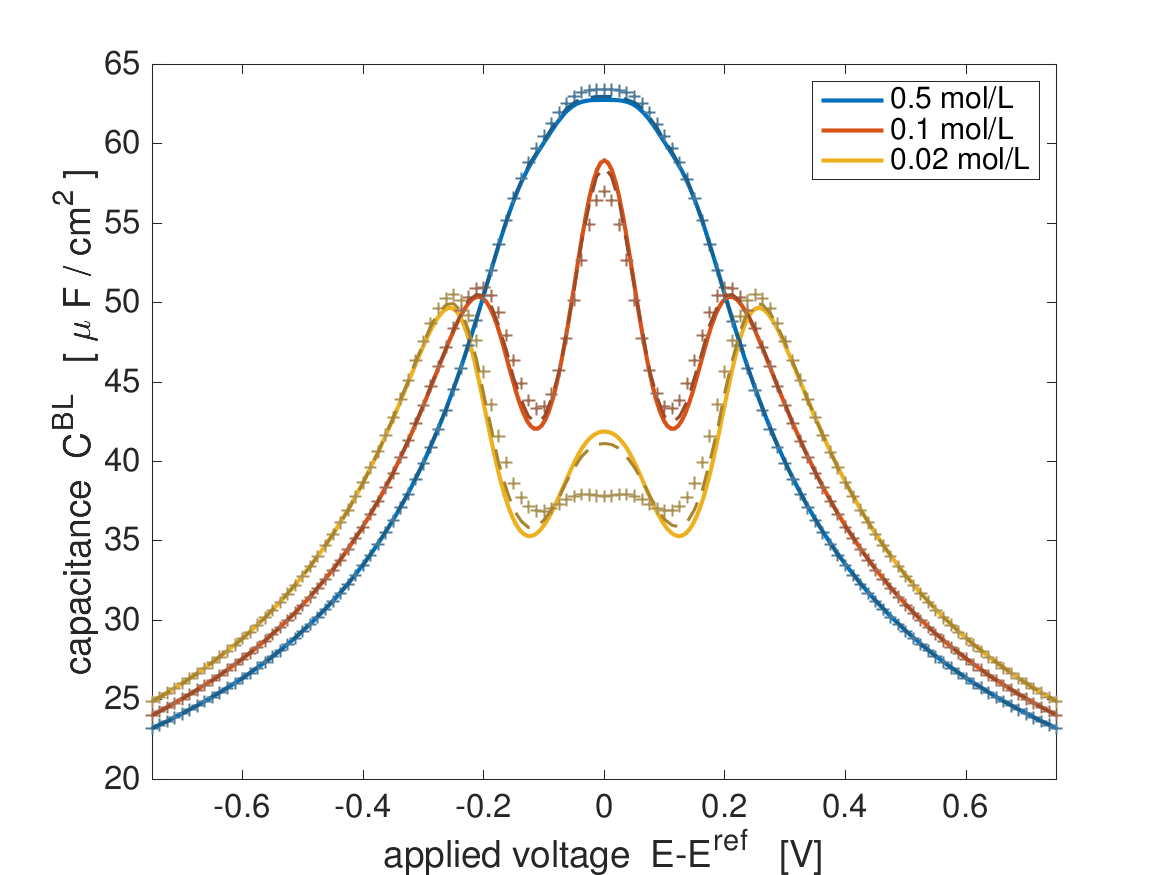
\includegraphics[width=0.45\textwidth]{c_2d_grain.pdf}
  \caption{Left: profile of the electrostatic potential for a bi-crystalline interface with different
    grain sizes.
    Right: double layer capacity curves for different electrolyte concentrations.
    Solid lines (—) refer to the weighted sum of the grain contributions.,
    (+) and dashed (- -) lines mark data obtained from numerical simulations for
    small and large grain sizes, respectively.
 \label{fig:JES}}
\end{figure}

%\begin{figure}
%  \centering
%  \includegraphics[width=0.5\textwidth]{ccfg.pdf}
%  \includegraphics[width=0.4\textwidth]{iceo.pdf}
%   \caption{Left and mid: time evolution of electrostatic potential and %concentration for
%  a unipolar Nernst-Planck-Poisson system with volume constraints. The concentrations $c$
%  stays in the physical limits $0<c<1$ \cite{CCFG2020}.
%  Right: induced charge electroosmotic flow over a floating electrode induced by a lateral
%  electric field \cite{FuhrmannEtAlECActa2019}. \label{fig:fv}}
%\end{figure}


\paragraph{Goals of the Project and Methodologies}
% Please include here:
% goals
% methodologies
Our recent results on modeling multi-material and polycrystalline metal-electrolyte interfaces are confined to the case of thermodynamic equilibrium without charge transfer reactions. This experimentally validated model framework is our starting point for non-equilibrium thermodynamic modeling of electron transfer reactions at multi-material electrodes coupled to charge transport in an electrolyte, taking into account  effects of polycrystalline interface structure, catalyst surface phase transitions, finite ion sizes, solvation, concentration dependent susceptibility.

In order to take into account  the heterogeneous structure of the interface, we aim at a transition from surface patch labeling towards a description %of a multi-material electrode in terms of  
on the basis of work function values of the multi-material electrode. This allows additionally for a statistical distribution across the surface. Further we intend to extend averaging methods as developed in \cite{JES}  by periodic and statistical homogenization approaches.
%
These efforts shall result in  rate   equations  for polycrystalline interfaces  and their respective coupling to the bulk processes.

Many eletrocatalysts, in particular platinum free electrocatalysts for water splitting, have semiconductor properties, therefore we intend to extend the electrode models to the case of semiconductor - electrolyte interfaces.

Thermodynamically consistent discretization approaches which allow to preserve qualitative features of the continuous systems of equations  (second law of thermodynamics, mass conservation, positivity of concentrations) will be used to  develop numerical simulation models for multi-material electrocatalytic systems.  Preferably, models will be implemented in  Julia.

Model adaptivity strategies shall provide efficient ways to handle the different temporal and spatial scales. % \eg double layer resolution vs. electro-neutrality condition. 
In particular they shall be able to decide between spatial resolution of the electrode boundary layers and the lumping of the relevant processes into interface models.

\paragraph{Main Contributions}
The envisioned modeling framework will allow to set up analytical and numerical simulation methods for multi-material electrocatalytic systems. The features include electrochemical measurement processes, e.g. voltage cycling for CV or extraction of potential surfaces for STM.
These simulation tools shall be used to create a series of prototypical synthetical measurement data, which can serve (i) as catalogue for experimentalists to (visually) compare their results to our modeling and simulation approach, (ii) as (labeled)  training sets for machine learning tools,  (iii) as database for parameter estimation. For our data we will use the infrastructure developed in the framework of the NFDI4Cat consortium under the German National Research Data Initiative (NDFI) \cite{NFDI4Cat}, provisionally allowing to access measurement data by other groups.

Further, the project will result in extended bulk-surface models for electrochemical systems which provide an ample field for further investigation in analysis and numerics. 
Classical electrode theory based on the Butler-Volmer equation will be generalized.  Upscaling and averaging methods for surface rate equations developed in the project are of potential interest in other applications.

Methodologies for consistent coupling of charge transport processes described by drift-diffusion systems and
corresponding numerical methods are investigated in several other projects of the application area AA2.

\paragraph{Future Research and New Horizons}
% Please consider the following aspects:
% - Describe the scientific novelties of the project compared to the state-of-the-art in the field of the project.
The establishment of material models for heterogeneously structured electrocatalytically active surfaces
provides the possibility of experimental comparison with polycrystalline or  multi-material electrodes
as they occur in electrochemical experimentation and in real world devices.

% - Highlight the long term research or application perspectives which will be opened by your project.
The ability to model and simulate processes at polycrystalline electrodes, and the communication pathway with experimentalists related to the publication of synthetic measurement data will be an excellent foundation
for collaborative research projects in the field of electrochemistry based e.g. on grants available through
the National Hydrogen Initiative.

% - Address potential future research questions / problem complexes which may be approached based on the results upon completion of the project work.
In the future, it will be possible to apply the methodology to various electrolyte-interface systems
and to set up inverse problems to interpret results of various measurement methods used to characterize real electrode surfaces. Upon experimental validation, the models can be used to optimize electrocatalytic processes.
The inclusion of semiconducting electrodes will be a starting point to develop models and simulation methods
for photocatalytic reactions.
The methodological framework and the resulting models will provide many open questions regarding their
mathematical and numerical analysis.


%\nocite{*} % remove this line if you only want to show cited references
\bibliographystyle{mathplusplainyr}
\bibliography{mybibfile}

% \bibliographystyleP{matheonplainyr}
% \bibliographyP{mybibfile}
% \bibliographystyleO{matheonplainyr}
% \bibliographyO{mybibfile}


% This is needed for multiple bib-files
% \printbibliography[heading=none]
% \printbibliography[keyword={reflist},heading=none]

\subsection*{Additional Aspects of the Proposal}

\paragraph{Collaborations}
% Please list existing or planned cooperation (scientific, industrial, ...),
% both internal and external. Sort as follows:

Internal cooperation (within MATH+)
\begin{itemize}
\item AA2: A. Glitzky  et al, P. Farrell et al, D. Hömberg et al: models and methods for Drift-Diffusion systems coupled
  to various physical processes
\item AA2: M. Radziunas: numerical method development
\item AA2: M. Thomas et al: Bulk-Interface models
\item AA2: S.Burger: development of outlook on photocatalysis
\end{itemize}

External scientific cooperation (outside MATH+)
%partially continuing the cooperation of the first phase (?)
\begin{itemize}
\item Dr. S. Matera, FU Berlin, UniSysCat
\item Prof. Dr. P. Strasser TU Berlin
\item Prof. Dr. Timo Jacob, University Ulm, Institute of Electrochemistry     
\item Prof. Dr. Michael Eikerling, Forschungszentrum Jülich
\item Dr. Peter Berg, University of Alberta
\item Prof. Boris Zaltzman, Ben Gurion University of the Negev
\end{itemize}

External industrial cooperation (outside MATH+): Robert Bosch GmbH, Dr. Ulrich Sauter, Modeling of Electrochemical Components (CR/ARC CE-MEC) 
%continuing the cooperation of the first phase (?)
%\begin{itemize}
%\item Robert Bosch GmbH, Dr. Ulrich Sauter, Modeling of %Electrochemical Components (CR/ARC CE-MEC) 
%\end{itemize}

\paragraph{Related Projects}
% Please include your funded projects which are topicwise related to this proposal.
% State the main differences.
\begin{itemize}
\item ``Electrical Double Layers in Solid Oxide Cells'' (DFG FU 316/14-1; PI J. Fuhrmann) focuses
  on high temperature solid electrolytes
\item ``Kontinuumsbasierte Modellierung und Simulation elektrochemischer Prozesse für Metall-Luft-Batterien''
  (BMBF  03EK3051B; PI J.Fuhrmann, M. Landstofer) focuses on homogeneous electrolyte models
\item ``Coupled atomistic and nanofluidic simulations for electrocatalysis'' (Joint PhD project with S. Matera
  in the  Berlin International Graduate School for Natural Science and Engineering (BIG-NSE) linked
  to the UniSysCat excellence cluster) focuses on atomistic electrode models
% Das muss meiner Meinung nach nicht unbedingt hier hin ...
%\item ``Modellbasierte Abschätzung der Lebensdauer von gealterten Li-Batterien für die 2nd-Life Anwendung als stationärer
%  Stromspeicher (MALLi$^2$)'' (BMBF 05M18BCA; PI: M. Landstorfer): General modeling and homogenization of battery cells
%  without phase separation.
\end{itemize}

\paragraph{Further Impact of the Project on MATH$+$}
% Please discuss different types of impact of your project on
% MATH+. Sort as follows:
% - Additional Funding (Further funding of research themes related to this project)
We see a good perspective for additional projects within the National Hydrogen Initiative. 
%funding based on the modeling and simulation approach
%developed in this project.
%
% - Research Training (Summer schools, etc.)
Methods and results of the project will be used in teaching activities at TU Berlin.
%
% - Gender and Diversity (Activities for female students, etc.)
Further we will participate education of a diverse group of people in the teaching activities
%
% - Complementary Skills (Opportunities for project staff to acquire skills complementing existing ones)
%
%Obtain further skills in numerical methods and their implementation, unique skills in electrochemical
Dr. Manuel Landstorfer intends to finish his habilition during the project. %modeling asked for in  industry
%
% - Outreach (Plenary lectures, public lectures, etc.)
We will participate in public outreach activities within the National Hydrogen Initiative. 

\paragraph{Position(s) of the PI(s)}
% It is required that the position(s) of all PIs is/are secured for the complete duration of the project applied for. PIs on a fixed-term contract should provide corresponding evidence through a statement by their supervisor (e.g. project proposal XY currently being reviewed/extended by third party funding agency ZZ). 
% Junior-Profs and Junior Research Group Leaders should refer to the envisioned date of their interim evaluation. 
Both PIs have full permanent positions at Weierstrass Institute, J. Fuhrmann is deputy head of WIAS RG3.

\end{document}
%%%%%%%%%%%%%%%%%%%%%%%%%%%%%%%%%%%%%%%%%%%%%%%%%%%%%%%%%%%%%%%%%%%%%%
